
%
%  PARA TRABALLOS EN GALLEGO USAR (LINEA 12): \usepackage[galician]{babel}
%  PARA TRABALLOS EN CASTELLANO USAR (LINEA 13): \usepackage[spanish]{babel}
%
% Para los acentos usamos codificacion UTF-8 (LINEA 10): \usepackage[utf8]{inputenc} 
% Si se usase la codificacion es_ES.ISO-8859-1 (LINEA 11): \usepackage[latin1]{inputenc}
% La conversion de acentos se hace con: iconv -f UTF-8 -t ISO-8859-1 filename.tex
%
% Como se incluyen figuras eps hay que compilar con: latex traballo , dvipdf traballo
%

\documentclass[12pt,twoside,a4paper]{book}
% pódense engadir todos os packages necesarios
\usepackage[spanish]{babel}

\usepackage{graphicx}
\usepackage[dvips]{epsfig}
\usepackage{amssymb}
\usepackage{eurosym}
\usepackage{float}
\usepackage{latexsym}
\usepackage{a4}
\usepackage{xcolor,colortbl}
\usepackage{listings}
\usepackage{pdflscape}
\usepackage{tikz}
\usepackage{multirow, array} % para las tablas
\usepackage{float} % para usar [H]
% \usepackage{hyperref} % menús no pdf pero non leva ben co package galician



\addto\captionsgalician{\def\contentsname{Memoria tipo A -- \'{I}ndice xeral }}
	

\begin{document}
\pagestyle{empty}
\begin{center}
	{\bf\Large UNIVERSIDADE DE SANTIAGO DE COMPOSTELA}
	
	\vspace{0.5cm}
	
\includegraphics[width=5cm]{figuras/logo_usc.eps}
	
	\vspace{0.5cm}
	{\bf\large ESCOLA TÉCNICA SUPERIOR DE ENXEÑARÍA}
	
	\vspace{2cm}
	{\bf\LARGE Sistema de alertas basado en procesamiento en tiempo real de logs en una plataforma con disponibilidad 24/7}
	
	%\vspace{0.5cm}
	%{\bf\LARGE Subtítulo do Traballo de Fin de Grao}
\end{center}

\vspace{2cm}
\hspace{4cm}\begin{tabular}{l}
	{\it\Large Autor/a:} \\
	{\bf\Large Adrián Bernárdez Cornes} \\
	~ \\
	{\it\Large Titores:} \\
	{\bf\Large Manuel Lama Penín} \\
\end{tabular}

\vspace{2cm}
\begin{center}
	{\bf\Large Máster universitario en Tecnologías de Análisis de Datos
Masivos: Big Data}
	
	\vspace{0.5cm}
	{\bf\large Julio 2022}
	
	\vspace{0.5cm}
	Traballo de Fin de Máster presentado na Escola Técnica Superior de Enxeñaría da Universidade de Santiago de Compostela para a obtención do Máster Interuniversitario en Big Data: Tecnologías de Análisis de Datos Masivos
\end{center}


\cleardoublepage

\cleardoublepage
\pagestyle{plain}
\tableofcontents
\listoffigures
\listoftables

% Agora incluimos os capítulos. Cambiamos a numeración e as cabeceiras
\cleardoublepage
\pagenumbering{arabic}
\setcounter{page}{1}
\pagestyle{headings}
\setlength{\parskip}{8mm}
\chapter{Introdución}
\hyphenation{In-te-re-se}

Para un sistema de máxima disponibilidad como es el caso de sistemas de dispensación farmacéutica,
los cuales deben estar en funcionamiento las 24 horas del día, los 7 días de la semana se generan una cantidad masiva de logs. Para cumplir con esta disponibilidad se deberá disponer de un equipo de desarrollo y de soporte que cubrirán todas las horas del día haciendo guardias durante las horas no laborables. Sin embargo, en caso de que un componente falle, el tiempo de respuesta en informar del problema y buscar una solución deberá ser el mínimo posible independientemente de la causa y circunstancia en que se de el problema.

El objetivo del proyecto será aportar una plataforma que se encargue de generar alertas en caso de una incidencia importante, analizando los logs de actividad hasta dar con el componente afectado. De esta forma el sistema deberá responder en tiempo real con el fin de agilizar el proceso y mejorar el servicio. Con esta nueva operativa se podría registrar estas alertas para poder dotar al equipo de un informe de las incidencias y sus componentes afectados, con el fin de elaborar soluciones a problemas comunes y poder formar de una manera más eficiente y exacta a los encargados del correcto funcionamiento del sistema principal. 

Un ejemplo de uso concreto sería la caída de una base de datos sobre la que opera la aplicación. En este caso se buscaría poder recibir una alerta lo antes posible con la información necesaria para la identificación del problema y su posible solución. Este tipo de sistemas se tienen que basar sus principios en:

\begin{itemize}
	\item Fiabilidad, la solución no deberán generar falsos positivos ni obviar problemas que suponen una alerta.
	\item Tiempo real, la información debe llegar al destino lo antes posible después de su generación.
	\item Adaptabilidad, la solución deberá estar desacoplada de la aplicación a monitorizar y será resiliente a cambios.
\end{itemize}

En la actualidad existen ciertas opciones que se adecúan en cierta medida, como puede ser el caso de elasticsearch y kivana o graylog. Sin embargo, las funcionalidades necesarias para cumplir la funcionalidad no forman parte de la licencia gratuíta de las aplicaciones, o la gestión de alertas (activadores y funciones) no es lo suficientemente flexible ni abarca aquellos eventos que se espera que realice la solución planteada.

Se buscará que la alerta generada sea lo más descriptible posible y que consiga dar un indicio de la causa del problema. De esta manera se podrá dar una respuesta con tiempos mínimos tiempos de espera, lo cual supondría tanto una mejora en el servicio como la facilitación del trabajo de cara al equipo encargado de la supervisión de la aplicación. A la hora realizar el diseño de la plataforma se deberá tener los siguientes puntos como claves: 

\begin{itemize}
\item Dada una aplicación que tenga una disponibilidad total y sobre la que opere un número elevado
de usuarios, se generan una cantidad de logs masiva, que en caso de que se produzca un error, el proceso de revisión de logs y la diagnosis posterior puede ocupar un tiempo
demasiado largo en caso de que no se pueden producir cortes en el servicio.

\item La finalidad del proyecto será disponer de una plataforma para detectar en tiempo real posibles problemas e incidencias y
clasificarlas según experiencias pasadas reducirá ese tiempo de espera en gran medida. La funcionalidad de la clasificación de la alerta entre problemas conocidos supondría una mejora significativa en la gestión operacional de la aplicación.

\item Registrar las incidencias alertadas de errores no conocidos supone un extra añadido, ya que se dispondrá de un histórico
con el que saldrán a la luz posibles bugs o errores frecuentes de cara a poder llevar un control
y análisis de la aplicación más exhaustiva.  

\item El proyecto deberá estar desacoplado de la aplicación principal y estar preparado para adaptarse a cambios y nuevas funcionalidades.

\item En caso de detectar un detectar errores desconocidos, de los cuales la aplicación no conoce la causa, se deberá implementar un sistema de obtención de anomalías en los logs para mostrar las excepciones causantes del error.

\end{itemize}




\section{Objetivos}

El objetivo general del proyecto será la implementación de una herramienta que permita la detección en near-real-time de incidencias en una aplicación a través de ficheros de log. La herramienta deberá clasificar estas incidencias mediante reglas configurables, y en caso de tratarse de una incidencia desconocida para el sistema se realizará una detección de anomalías con el fin de descubrir la causa de la incidencia.

Una vez planteado el contexto se identifican los siguientes objetivos a más bajo nivel:

\begin{enumerate}
	\item \textbf{Emisión de alertas en Near Real Time con información relevante tras la detección de posibles errores o
incidencias. Se buscará enviar la posible causa del problema raíz:} El principal objetivo del proyecto es la construcción de una plataforma con las herramientas necesarias para la emisión de alertas tempranas en caso de producirse una incidencia en la aplicación a monitorizar. Se espera que la alertas se generen en near real time con el fin de una recuperación del servicio los más rápida y eficiente posible. La plataforma deberá ser configurable ya que nace de la necesidad de coexistir servicio a un sistema con disponibilidad total que está en continuo desarrollo y evolución.
	\item \textbf{Registro de las incidencias encontradas con la información necesaria para su posterior
tratamiento:} Se deberá llevar un registro de las incidencias detectadas de errores no identificados y de los logs de la aplicación obtenidos. De esta forma una vez solucionada la incidencia se podrá catalogar y registrar los errores producidos en la aplicación con el fin de un análisis posterior en el que se podrán detectar posibles vulnerabilidades o bugs.
	\item \textbf{Clasificar el error mediante los logs de la aplicación:} La plataforma deberá clasificar de la incidencia en base a los logs producidos en la aplicación. De esta forma se podrá plantear el envío de los pasos conocidos para su solución en cuanto se detecte el error. En caso de que se trate de un error no conocido se aplicarán técnicas de Machine Learning para la obtención de anomalías en los registros.
\end{enumerate}
	


\section{Alcance}

La solución alcanzada deberá cumplir los objetivos definidos en el apartado anterior. Por un lado la plataforma a desarrollar deberá incorporar las herramientas necesarias que permitan de forma simple para un usuario la creación de alertas y modificación de las mismas en base a criterios acordados y a la experiencia obtenida. Por otro deberá utilizar los datos obtenidos con la finalidad de aplicar herramientas de Machine Learning con el fin de obtener la información más útil para la solución de la incidencia.

Se deberá tener en cuenta que no se podrán utilizar datos reales de la aplicación actual debido a que se estarían utilizando datos personales de terceros lo que incumpliría la normativa de protección de datos. En su lugar se utilizarán logs de entornos de desarrollo sobre los cuales se implementará una solución que permita crear un escenario equivalente al entorno real sin datos personales y a menor escala.

Una vez finalizado el desarrollo se deberá proporcionar una plataforma que pueda ser agregada a la aplicación actual y que deberá ser validada a posteriori. Para ello deberá proponerse una arquitectura como una extensión de la plataforma actual con el fin de que coexista. Por ello se ha de tener en cuenta que la instalación y despliegue será controlado en un entorno preparado para este fin permitiendo un control de versiones y registro del resultado.

Como entregables del proyecto serán los siguiente:
\begin{enumerate}
\item Plataforma encargada de la emisión de alertas con reglas de alertas configurables.
\item Plataforma encargada de la clasificación de las incidencias y su registro.
\item Propuesta de integración en el sistema real
\end{enumerate}
\cleardoublepage
\chapter{Revisión de soluciones comerciales}

\section{Gestión de alertas}

La monitorización de la actividad en aplicaciones puede ser un trabajo tedioso, sin embargo existen buenas razones pare hacerlo. Se puede llevar a cabo por motivos muy variados como buscar e investigar inicios de sesión sospechosos en estaciones de trabajo, visualizar dispositivos conectados a redes y servidores o identificar las posibles deficiencias o bugs en el sistema. 

Debido a esta serie de problemáticas, existen un número considerable de registro de código abierto y herramientas de análisis disponibles en la actualidad, lo que hace que elegir los recursos adecuados para los registros de actividad sea un trabajo considerable. La comunidad de software de código abierto y gratuito ofrece diseños de registros que funcionan con todo tipo de sitios y prácticamente con cualquier sistema operativo. 

En esta sección se tratará de analizar los productos y herramientas existentes enfocados al tratamiento de log con el fin de averiguar si cumplen con los requisitos planteados o si pueden resultar una ayuda de cara a la implementación de la solución.

\subsection{Graylog}

Graylog comenzó en Alemania en 2011 y ahora se ofrece como una herramienta de código abierto o una solución comercial. Está diseñado para ser un sistema de administración de registros centralizado que recibe flujos de datos de varios servidores o puntos finales y le permite navegar o analizar esa información rápidamente.

Graylog dispone de las siguientes funcionalidades:

\begin{itemize}
\item \textbf{Recolección y procesado de logs}: implemente la necesidad de leer distintos tipos de logs de distintas fuentes para ser tratados de forma descentralizada, así como la posibilidad de integración con directorios LDAP.

\item \textbf{Transformación de datos}: ofrece la posibilidad de transformar los datos de entrada para publicador a otras aplicaciones como fuente de datos refinada.

\item \textbf{Análisis e investigación}: proporciona la capacidad para buscar y analizar información  de distintas fuentes de datos en una única consulta.

\item \textbf{Grafos y estadísticas}: dispone de múltiples gráficos para analizar los datos de forma sencilla accesibles mediante interfaz web.

\item \textbf{Alertas}: provee de la capacidad de crear disparadores y acciones que se activen cuando se produce un evento determinado en los logs. 
\end{itemize}

La arquitectura está compuesta por una serie de nodos que se encargan de leer la información de las máquinas a monitorizar y enviarla a los nodos de Elastic Search que almacenan y procesan todos los logs y mensajes recibidos. Para almacenar los metadatos se utiliza MongoDB y finalmente se proporciona una interfaz web para visualizar los datos recolectados y procesados.


\subsection{Nagios}

Nagios comenzó con un solo desarrollador en 1999 y desde entonces se ha convertido en una de las herramientas de código abierto más confiables para administrar datos de registro. La versión actual de Nagios puede integrarse con servidores que ejecutan Microsoft Windows, Linux o Unix.

Su producto principal es un servidor de registros, cuyo objetivo es simplificar la recopilación de datos y hacer que la información sea más accesible para los administradores del sistema. El motor del servidor de registro de Nagios capturará datos en tiempo real y los enviará a una poderosa herramienta de búsqueda. La integración con un nuevo punto final o aplicación es fácil gracias al asistente de configuración integrado.

Nagios se usa con mayor frecuencia en organizaciones que necesitan monitorizar la seguridad de su red local. Puede auditar una variedad de eventos relacionados con la red y ayudar a automatizar la distribución de alertas. Nagios incluso se puede configurar para ejecutar scripts predefinidos si se cumple una determinada condición, lo que le permite resolver problemas antes de que un humano tenga que involucrarse.

Como parte de la auditoría de red, Nagios filtrará los datos de registro según la ubicación geográfica donde se originan. Eso significa que puede crear paneles de control completos con tecnología de mapeo para comprender cómo fluye su tráfico web.

\subsection{ELK Stack}
\label{sec:elk_stack}
\textbf{ELK Stack} o Elastic Stack es un proyecto OpenSource multiplataforma que abarca una serie de productos y soluciones que tienen como finalidad facilitar al usuario el tratamiento de la información. Se trata de una de las herramientas de código abierto más populares entre las organizaciones que necesitan examinar grandes conjuntos de datos y dar sentido a los registros de su sistema. Las funcionalidades básicas serían la de extraer, buscar, analizar y visualizar datos en tiempo real o de forma asíncrona.

ElasticSerch proporciona distintas formas de implementación, tanto de forma local e una única máquina o de forma distribuida utilizando un modelo SaaS (Software as service).

Su oferta principal se compone de tres productos separados correspondientes con sus tres siglas: Elasticsearch, Kibana y Logstash:

\begin{figure}[H]
\centerline{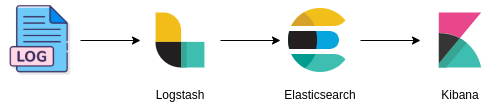
\includegraphics[width=15cm]{figuras/elkstack.png}}
\caption{Componentes del ELK Stack}
\label{enlace1}
\end{figure}

Como breve resumen de los elementos mostrados en la imagen serían:
\begin{itemize}
\item \textbf{Logs:} logs en el servidor que serán analizados e identificados.
\item \textbf{Logstash:} recoge logs y eventos que puede parsear y transformar.
\item \textbf{ElasticSearch:} almacena la información recogida por logstash y la indexa.
\item \textbf{Kibana:} se encarga de explorar, visualizar y compartir los datos almacenados en ElasticSearch.
\end{itemize}

\subsubsection{ElasticSearch}

ElasticSearch es el componente principal de ELK Stack, que presenta como principal responsabilidad las operaciones de catalogar y almacenar información que podrá se recuperada a posteriori de forma flexible. Se trata de un motor de búsqueda OpenSource distribuido y escalable basado en Apache Lucene, que incluye su propio lenguaje de consulta denominado Query DSL. 

Ofrece una API de tipo RESTful Json y clientes para distintos lenguajes de programación de forma oficial, al mismo tiempo que al ser una herramienta OpenSource dispone de una comunidad de usuarios que ofrece clientes y soporte para los lenguajes a los que no se les proporciona oficialmente.

ElasticSearch utiliza índices para registrar los documentos. Un índice de ElasticSearch se define como una colección de documentos que presentan relación entre sí. Elasticsearch almacena los datos como documentos JSON. Elastic Search utiliza una estructura de datos llamada índice invertido, el cual está diseñado para permitir búsquedas de texto de manera muy eficiente. Un índice invertido hace una lista de cada palabra única que aparece en cualquier documento e identifica todos los documentos en las que ocurre determinada palabra. Durante este proceso de indexación, Elasticsearch almacena documentos construyendo el índice invertio para poder buscar dastos en el documento casi en tiempo real.



\subsubsection{LogStash}

El componente LogStash  se encarga de procesar la información en crudo con el fin de que pueda ser consumida y almacenada por un motor de búsqueda, en concreto en el caso de ELK Stack será ElasticSearch. Se estructura en forma de pipeline con 3 secciones bien diferenciadas:

\begin{enumerate}
\item \textbf{Entrada (input):} conectores e interfaz necesaria para la recepción de datos en crudo de varias fuentes.
\item \textbf{Proceso y filtros (parse):} en esta sección se procesa la información obtenida en un forma comprensible y manejable por un motor de búsqueda. Las transformaciones se basan en filtros con funciones para convertir los datos.
\item \textbf{Salida (output):} conector de salida de la información procesada tras el filtrado. Por defecto la salida será ElasticSearch pero ofrece conexiones para otras plataformas.
\end{enumerate}

\subsubsection{Kibana}

El elemento restante del stack es Kibana, que proporciona la interfaz gráfica con la función de monitorizar. Se encarga de leer la información de ElasticSearch para después presentarla a través de una interfaz web donde se visualizará el contenido almacenado en el motor de búsqueda.

Dispone de gran variedad de gráficas, métricas histogramas y visualizaciones configurables que permiten analizar la información. Se basa en node.js y se trata de un cliente web multiplataforma OpenSource que podrá ser ejecutada en multitud de plataformas.


\subsection{Conclusiones}

Las herramientas mencionadas en esta sección proporcionan parte de la funcionalidad que se busca con este proyecto, sin embargo no consiguen todos los objetivos propuestos. Esto no quita que se pueda utilizar parte de la funcionalidad propuesta por la herramienta con el fin de construir la solución final del proyecto. Tras el análisis realizado de posibles herramientas existentes en el mercado se ha decidido eliminar GrayLog ya que se parte del requisito de que la solución deberá utilizar productos OpenSource, y en este caso la licencia gratuita de GrayLog solo permite el tratamiento de 2 GB diarios, lo cual no es lo suficiente para una aplicación como sobre la que va a actuar el proyecto. Por otro lado, Nagios no dispone de una licencia OpenSource y se descarta por este motivo.

Finalmente se ha optado por utilizar ELK Stack debido a la extensa documentación y comunidad, así como su posibilidad de escalado y a la rapidez de búsqueda gracias al indexado de la información. Utilizando las últimas versiones de kibana se podría utilizar las herramientas de gestión de alertas para la generación de eventos, sin embargo, esto no entra dentro de la licencia OpenSource y los triggers que dispone son limitados. El uso del \textbf{índice invertido} de ElasticSearch se espera que acelere las búsquedas por términos en gran medida, y en el caso real del proyecto se buscarán todas los documentos asociados a un id que se presenta dentro de cada línea de log, por lo tanto se esperan búsquedas muy rápidas y eficientes.

Debido a que existe una gran comunidad de usuarios de Elastic Search, se han creado de forma OpenSource un serie de plugins y complementos que mejoran el uso y proporcionan herramientas que con la funcionalidad stock no dispondríamos. Gracias a ello para la gestión de alertas se podrá utilizar la herramienta ElastAlert, que se trata de una solución totalmente Open Source creada como complemento a ElasticSearch para suplir las limitaciones presentes a la hora de alertar sobre eventos en los datos. Esta herramienta supone una gran ventaja ya que presenta una libertad total a la hora de crear acciones sobre las alertas generadas.

De esta forma aun teniendo que emplear tiempo en el conocimiento de las funcionalidades de las soluciones escogidas, será más eficiente que desarrollar una herramienta desde 0. Así se podrá asignar mas tiempo a los objetivos específicos del proyecto.
\cleardoublepage
\chapter{Propuesta de solución}


Los archivos de registro de actividad que sobre los que se obtendrá la información del sistema se dividen en varios archivos, cada uno con un objetivo concreto. En concreto se monitorizarán tres ficheros, los cuales poseen un ciclo de vida que consiste en pasar por un fichero plano, para una vez alcanzado un tamaño determino comprimirse y guardarse como histórico. Si el histórico tiene una antigüedad superior a los días establecidos como máximo se enviarán a un servidor que funcionará como almacenamiento. Estos tres ficheros tienen los siguientes acometidos:

\begin{itemize}
\item Registro de interacciones (peticiones y respuestas) con otros sistemas externos e internos.
\item Registro de las transformaciones y cálculos que reciben los datos en los distintos servicios de los que se compone la aplicación.
\item Registro de la aplicación de entrada que utilizarán los usuarios finales con registro de las operaciones solicitadas y pantallas accedidas.
\end{itemize}

En los logs de actividad se registrarán el momento en que se registran, la clase en la que se originó el comportamiento y el texto con la información que se está registrando en ese momento. 

Estos ficheros se unificarán en un único índice de ElasticSearch por un motivo en concreto: todos los registros de actividad tienen asociado un identificador de operación, es decir, cuando se intenta hacer una operación sobre la aplicación los logs de actividad generados desde el origen hasta el final tendrán asociado un identificador numérico. De esta forma se podrá obtener rápidamente con una única búsqueda sobre ElasticSearch todos los registros de operación asociados a una operación en concreto.


En este capítulo se va a describir la plataforma implementada para la emisión de alertas. La arquitectura diseñada para la plataforma es la siguiente:

\begin{figure}[H]
\centerline{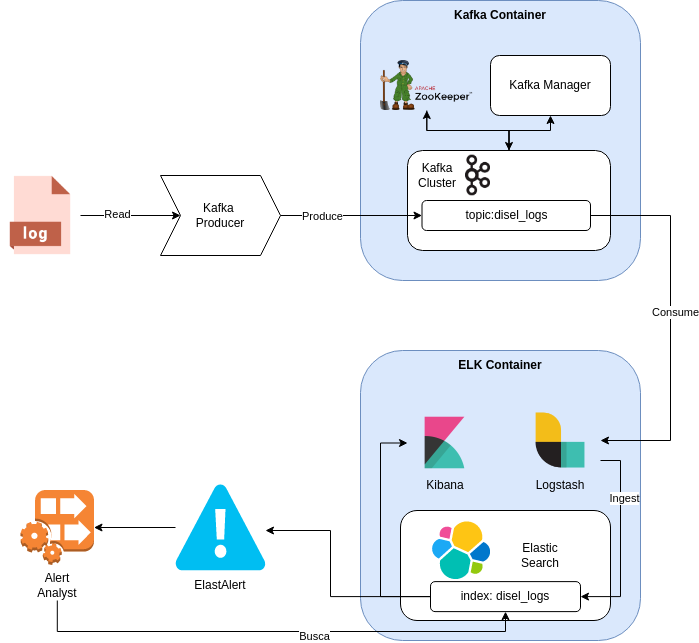
\includegraphics[width=15cm]{figuras/arquitectura.png}}
\caption{Arquitectura de la Plataforma de Gestión de Alertas}
\label{enlace1}
\end{figure}

La arquitectura estará compuesta por distintos componentes desplegados cada uno en un contenedores Docker. Se pueden distinguir las siguientes partes:

\begin{itemize}
\item \textbf{Producer}: como se ha comentado en el capítulo de introducción no es posible utilizar los logs de la aplicación real en el entorno de producción ya que se estaría incumpliendo la ley de protección de datos. Para ello se utilizarán logs ya registrados de los que se tiene certeza que se produjo una incidencia pero procedente de un entorno de desarrollo con datos que no contengan información sensitiva. Para reproducir el comportamiento de la aplicación se implementará un productos python que se encargue de leer cada línea de log y trasladarla a kafka, de esta forma replicará el comportamiento de escribir registros a lo largo del tiempo. Esto productos deberá poder comportarse de forma distinta para poder realizar todas las ingestas de datos necesarias para la realización de pruebas.

\item \textbf{Kafka server}: se utilizará kafka con el fin de trasladar los datos producidos en el productos al ELK Stack. La plataforma Apache Kafka es un sistema de transmisión de datos distribuido con capacidad de escalado y tolerante a fallos. Gracias a su alto rendimiento permitirá transmitir datos en tiempo real utilizando el patrón de mensajería publish/subscribe. 

\item \textbf{ELK Stack}: conjunto de aplicaciones (Elastic Search, Logstash y Kivana). Permite recoger datos de cualquier tpo de fuente y cualquier formato para realizar búsquedas, análisis y visualización de los datos en tiempo real. En la arquitectura planteada se para la aplicación real se obtendrán los datos a partir de ficheros de logs mediante Logstash y se almacenarán en el motor de búsquedas y análisis de Elasticsearch. Además, se permite la visualización, monitorización y explotación de datos en tiempo real mediante kibana.

\item \textbf{Generador de alertas}: este componente se encargará de la emisión de alertas utilizando para ello herramienta open source Elasticsearch, que se integra con ELK y permite detectar anomalías e inconsistencias en los datos. El conjunto de herramientas de \textbf{ELK (Elastic Stack)} más ElastAlert permite crear un sistema de monitorización para la extracción, almacenamiento y explotación de los datos de los procesos o sistemas a monitorizar. Además de esta herramienta se configurará en el mismo conector el proceso de reducción de logs, envío de emails y registro en base de datos.

\end{itemize}

En el sistema real se espera que las alertas se registren en la base de datos del sistema, sin embargo en el proyecto se utilizará un base de datos mongoDB desplegada en un contenedor Docker adicional.

\subsection{Generador de alertas}

Para detectar y emitir alertas como se comentó en el apartado anterior se utilizará ElastAlert.

ElastAlert es un componente originalmente diseñado por Yelp que es capaz de detectar anomalías, picos u otros patrones de interés. Se trata de un producto \textit{production-ready} y es un estándar de alerta conocido y aceptado dentro del ecosistema de ElasticSearch. En la documentación se especifica que "Si puede verlo en Kibana, ElastAlert puede alertarlo". ElastAlert podrá realizar distintas operaciones dependiendo que como se configuren las reglas en los ficheros de configuración. 

ElastAlert consulta periódicamente a ElasticSearch y los datos se trasladan al tipo de regla, la cual determina cuando se encuentra una coincidencia. Cuando se produce una coincidencia, se envía a una o más alertas que toman medidas en función de la coincidencia. Esto se configura mediante un conjunto de reglas, cada una de las cuales define una consulta, un tipo de regla y un conjunto de alertas. Se podrán definir tipos de regla del estilo:

\begin{itemize}
\item \textbf{Frequency}: existen una serie de X eventos en un tiempo Y. (Mismos códigos de error en un minuto)
\item \textbf{Spike}:la tasa de eventos aumenta/disminuye. (Número de peticiones por minuto sobre una operación concreta aumentan considerablemente) 
\item \textbf{Flatline}: menos de X eventos en Y tiempo. (No se realizan un mínimo de consultas a la bbdd en 1 minuto)
\item \textbf{Blacklist/Whitelist}: cuando un determinado campo coincide con una lista negra. (Se establecen unos códigos asociados a la indisponibilidad del sistema y en caso de detectarse se genera la alarma).
\item \textbf{Any}: cualquier evento que coincida con un filtro dado (Un código de error al que se le dará un trato especial).
\item \textbf{Change}: un campo tiene dos valores diferentes dentro de un tiempo (Una medida asociada a la temperatura varía drásticamente en un tiempo determinado´).


\end{itemize}

En la solución propuesta se distinguirán dos tipos de alertas principales definidas tras un estudio de los logs.

\begin{itemize}
    \item \textbf{Errores conocidos}: en la aplicación se pueden dar ciertos errores relativos a problemas de comunicaciones con otros servicios, caídas de los propios servicios así como problemas de conexión o caída con las bases de datos. Cuando se produce un error de este tipo la mayoría de operaciones van a devolver en la respuesta un código de ERROR del cual se puede obtener la información necesaria para su diagnóstico.
    
    Para este tipo de errores se generara una lista de reglas con un comportamiento similar:
    \begin{enumerate}
        \item Se detectará que se está repitiendo un código de error un número configurable de veces en un tiempo determinado.
        \item Cada regla tendrá asignado un diagnóstico y las acciones a seguir en cada caso.
        \item Se enviará un correo especificando el error detectado, el diagnóstico y los pasos a seguir al correo de notificación de incidencias.
        
    \end{enumerate}
    
    \item \textbf{Errores desconocidos}: por otro lado pueden darse errores desconocidos en la aplicación. Estos al contrario que los anteriores no tienen un fácil diagnóstico ni hay una serie de acciones por defecto a seguir. Se puede tratar de un gran abanico de posibilidades a la hora de buscar la causa, desde un mal tratamiento de una respuesta de un sistema o un bug que se introdujo en el código. 
    
    En este tipo de errores se buscará realizar un tratamiento de los logs aplicando Machine Learning para detectar anomalías que puedan ayudar al responsable a diagnosticar y buscar una solución. En este caso se definirá un regla, que en caso de detectar un error no definido obtenga el identificador de la transacción de la operación y haga una llamada al servicio del componente de Alert Analist con el fin de que trate los logs obtenidos.
    
\end{itemize}

El punto más importante que hace que ElastAlert sea la herramienta escogida es la posibilidad de realizar acciones totalmente configurables una vez se active un trigger. Para el proyecto interesa el hecho de para una misma alerta poder enviar un correo informando del problema, el registro en base de datos y ejecutar el proceso de reducción de log en caso de que se trate de un error desconocido.


\subsubsection{Reducción de log}

Cuando la aplicación falla con un error indeterminado se genera un log distinto al normal. Encontrar la causa del error puede ser un trabajo muy tedioso ya que involucra el estudio de los logs para encontrar la fracción del registro que se escapa de la operativa normal. Para hacer esta tarea más simple se utilizará LogReduce, el cual es un librería de código abierto que permite la generación de modelos Machine Learning entrenándolo con ejecuciones exitosas de procesos anteriores para extraer anomalías de los registros de ejecuciones fallidas.

Los logs de la aplicación se componen de un registro de los distintos servicios que permite la aplicación. Cada vez que un servicio es invocado se guardará un registro de la petición, las transformaciones realizadas sobre los datos, información referente a las casuísticas concretas y de la respuesta. El conjunto de los registros comunes en la ejecución de un servicio que finalice correctamente se conocerá como \textbf{\textit{Basenile}}.  En caso de se produzca algún tipo de error durante la ejecución del servicio se producirán excepciones que ayudarán a definir la causa del fallo.


Para eliminar los \textit{Baselines} de un log errado se podrá utilizar un algoritmo de k vecinos más próximos (\textbf{k-nearest neighbors pattern recognition algorithm k-NN}). 

Para ello, cada evento registrado en el log deberá ser convertido a un valor numérico aplicando algoritmos de Hashing Vectorizer. De esta forma se consigue mapear cada palabra y codificar cada evento en una matriz dispersa. Para mejorar este proceso se deberá aplicar una limpieza del texto quitando stop-words (palabras que no tienen significado por si solas), así como un proceso de tokenización para eliminar datos aleatorios como IPs y marcas temporales.

Una vez el modelo esté entrenado se podrá calcular la distancia de cada evento con respecto al \textit{Baseline} y mostrar aquellos resultados con un valor de distancia mayor que un umbral fijado. 

\begin{figure}[H]
\centerline{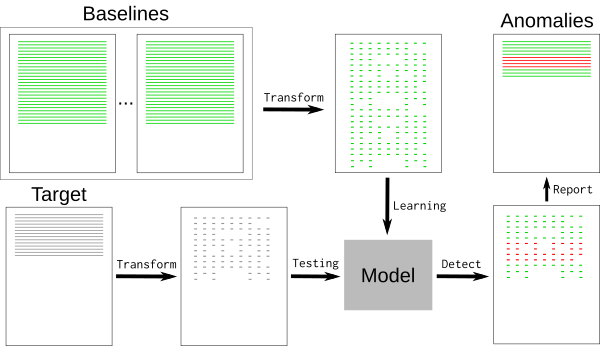
\includegraphics[width=15cm]{figuras/logreduce.png}}
\caption{Pipeline logreduce}
\label{enlace1}
\end{figure}

La librería LogReduce implementa este proceso con las ventajas de que se pueden especificar múltiples \textit{Baselines} para entrenar el modelo, así como la generación de reportes html para la mejor visualización del proceso.

El proceso de entrenamiento por tanto podrá ser cíclico de forma que en la que se vayan generando nuevos \textit{Baselines} añadirlos a la construcción del modelo. De esta forma el modelo estará preparado para cambios y evolucionará de igual manera que lo hace la aplicación. 


\cleardoublepage
\chapter{Pruebas}

Con el fin de comprobar el correcto funcionamiento de la solución se realizarán distintas pruebas para corroborar que las alertas se generan correctamente y en un tiempo que pueda ser comprendido dentro de un sistema near real time. Para ello se obtendrá un conjunto de logs correctos y errores que se querrá identificar como una alerta (tanto de un error conocido con un error desconocido) con el objetivo de forzar la generación de una alerta con la que comprobar que se recibe dentro del margen temporal esperado.

Debido a esto será necesario un trabajo previo de separación de logs en operaciones con errores y operaciones con funcionamiento correcto. Esto se llevará a cabo con un script Python, que separará en ficheros los dos tipos de operaciones a partir de logs producidos en un entorno no productivo de la aplicación. Una vez realizada la separación se podrá replicar el comportamiento de la aplicación a monitorizar, para lo que se desarrollarán dos scripts Python con las siguientes funciones:

\begin{itemize}
\item Script de carga inicial que permita una ingesta de datos hasta el tamaño deseado en Elastic Search. Para controlar el tamaño de datos cargados en Elastic se podrá utilizar el comando:

\begin{verbatim}
curl 'elasticsearch:9200/_cat/indices?v' 
-H "Authorization: Basic ********************"
\end{verbatim}

\item Script que permita la publicación de logs en Kafka que reciba como entrada la cantidad de operaciones que se publican por segundo, el número de operaciones correctas que se publicarán hasta que se envíe el error y el tipo de error (conocido o desconocido).
\end{itemize}

Con esto conseguimos proporcionar el estado de alarma bajo demanda y así poder comprobar la respuesta en distintas situaciones.

También interesa medir si se la información obtenida de aplicar la detección de anomalías sobre la traza de logs de errores desconocidos se considere útil. Para ello una vez obtenida la alerta en el informe generado deberá estar resaltado aquellas líneas de log que en un trabajo previo se han clasificado como las que contienen la causa de la incidencia.`

\section{Pruebas de Alertas y Rendimiento}

Para comprobar que las alertas aportan una ayuda y mejora al sistema real, se deberá probar que efectivamente se generan las alertas y se definirá un máximo de tiempo desde que se produce la incidencia hasta que el sistema la notifica. Se ha de tener en cuenta que se está trabajando sobre un prototipo que no corre sobre un sistema en producción, por lo que debido a la menor capacidad de computo será complicado generar un número semejante de logs por segundo que el sistema real, sin embargo, se esperarán tiempos inferiores a 5 minutos entre el registro de la incidencia en los logs y la generación de la alerta. Se probarán distintos números de logs generados por segundo que sirva de estimación de comportamiento en el sistema real, así como distintos números de reglas de alertas desplegadas.

Con la realización de las pruebas se intentará conseguir tres objetivos:

\begin{itemize}


	\item \textbf{Ejecución correcta}: Se deberá comprobar que efectivamente se genera una alerta cuando se produce una incidencia en el sistema. Para que esto se considere correcto deberá generarse siempre una alerta en cada uno de los casos de prueba propuestos.

	\item \textbf{Obtención de la alerta en Near Real Time}: en caso de que el primer punto se valide correctamente, también se ha de comprobar el tiempo que transcurre desde que se genera la incidencia (en este caso mockeandola) hasta que la alerta es recibida es inferior al tiempo estimado.

	\item \textbf{Medida de recursos utilizados}: ya que los distintos componentes de la solución estarán desplegados en docker se deberá comprobar como afecta una escalada en el las cantidades de logs a analizar con el fin de estimar que recursos serían necesarios para poder tratar con el sistema real. Se tomará de medida el uso de CPU y memoria.

\end{itemize}

Para cada una de las pruebas con distintos número de reglas desplegadas se realizará el siguiente procedimiento:

\begin{enumerate}
	\item Despliegue de los contenedores Docker con la configuración y sin datos cargados.
	\item Para cada prueba individual se realiza la ingesta inicial de los datos   hasta el tamaño propuesto.
	\item Ejecución del script que genera la alarma con números distintos de reglas desplegadas.
	\item Registro de tiempos de respuesta y de recursos utilizados en los contenedores.
	\item Los puntos 4 y 5 se repetirá unas 5 veces y se calculará la media de los tiempos.
\end{enumerate}


Con el fin de comprobar como afecta el número de reglas que se tengan desplegadas se repetirán las pruebas con un número distinto y así establecer una aproximación de los recursos utilizados con varias pruebas. Además para facilitar el proceso durante las pruebas se establecerá que las alertas se ejecutan cuando se encuentre el primer error especificando con los parámetros:

\begin{verbatim}

# (Required, frequency specific)
# Alert when this many documents matching the query occur within a timeframe
num_events: 1

# (Required, frequency specific)
# num_events must occur within this amount of time to trigger an alert
timeframe:
    hours: 1
    
\end{verbatim}


\subsection{Muestra de los datos}

En la primera gráfica se mostrará la media de los tiempos obtenidos frente a los datos cargados en elastic search.

\begin{figure}[H]
\centerline{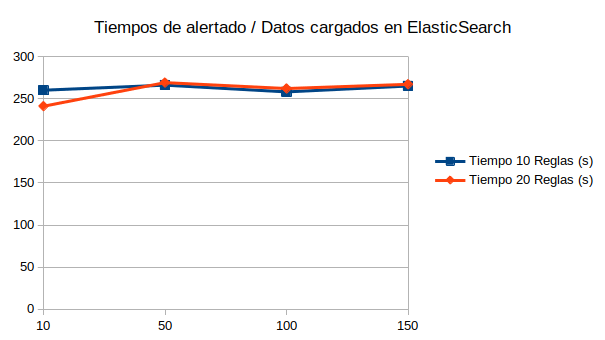
\includegraphics[width=15cm]{figuras/GraficaTiempos.png}}
\caption{Gráfica de tiempos}
\label{enlace1}
\end{figure}

Como podemos observar un aumento substancial en la cantidad de datos de elastic search no supone un aumento significativo del tiempo de alerta. Tratándose de una POC en un entorno limitado el resultado obtenido supera con creces a lo esperado. Se puede esperar que en un entorno productivo el sistema funcione dentro de un rango de tiempo que suponga una mejora en el sistema de monitorizado. 

Por otro lado el consumo de recursos dependiendo del número de reglas es el siguiente:

\begin{figure}[H]
\centerline{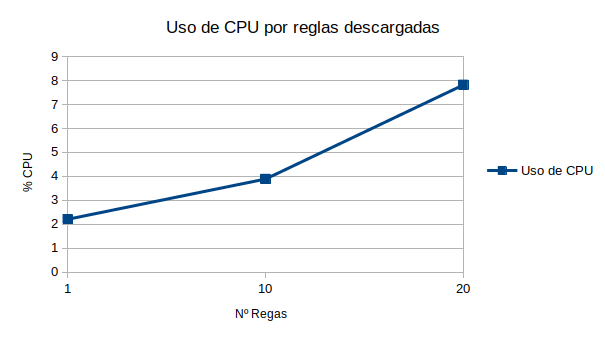
\includegraphics[width=15cm]{figuras/GraficaRecursos.png}}
\caption{Gráfica de recursos}
\label{enlace1}
\end{figure}

Como se puede observar un aumento del número de reglas si que implica un uso mas exhaustivo de los recursos. Sin embargo, el uso de CPU se mantiene relativamente bajo e incluso probando con un número de reglas mayor al esperando en entornos productivos el uso de CPU no supera umbrales preocupantes.


\subsection{Conclusiones}

Una vez realizado el proceso de pruebas sobre el sistema se puede afirmar lo siguiente:

\begin{itemize}

\item El sistema cumple con la fiabilidad y tiempo esperado dentro de un entorno de pruebas acotado al hardware disponible.

\item Un aumento drástico en la cantidad de datos cargados en Elastic Search no supone una peor prestación en cuanto a tiempos de alertado.

\item El aumento de número de reglas no supone peores tiempos de alertado, aún que si que se puede percibir un pequeño mayor consumo de recursos. 

\end{itemize}

\section{Pruebas del detector de anomalías en errores desconocidos}

Como objetivo secundario de la aplicación se buscará probar que para los errores desconocidos se proporciona una herramienta que pueda ayudar a la resolución de la alerta.

Para esta prueba se han buscado operaciones fallidas con un error desconocido en las que se distinguieron claramente la causa del error. En este caso varias operaciones en las que se produjo una excepción java no controlada que llegó a registrarse.

Por otro lado, se realizará un entrenamiento inicial del modelo utilizando un conjunto logs de resultados correctos de la operación a probar. Para ello se utilizarán los logs utilizados en las pruebas de rendimiento y se filtrarán por operaciones para entrenar un modelo por operación. Una vez entrenados los modelos y aplicada la detección de anomalías se genera un informe que resalte aquellas líneas que difieran de las líneas base. Para ello se utilizarán las funcionalidades de la librería \textit{LogReduce} comentada en el apartado \hyperref[sec:log_reduction]{\textit{Reducción de log}}.

Se definirá como línea clasificada como anomalía aquellas en las que se calcule una distancia al baseline explicado en el apartado anterior superior a 0,5. Una correcta clasificación se dará cuando se detecte como anomalía una línea con información sobre el error. 

Lo que se busca con esta funcionalidad es que se intente limpiar correctamente los logs, sin embargo, debido a la naturaleza del sistema a monitorizar se dará más importancia a que no se obtengan falsos negativos (líneas clasificadas como no anomalías, pero que si lo son). En las pruebas realizadas no se han obtenido más de 10 falsos negativos por lo que la limpieza se puede considerar lo suficientemente correcta. 

El resultado se considera correcto, ya que se efectivamente la gran mayoría de las líneas causantes del problema se resaltan como anomalías, sin embargo, no es un resultado perfecto, ya que también se están obteniendo falsos positivos de anomalías (aunque con un valor de diferencia menor) debido al gran número de caminos y posibilidades posibles en las operaciones. Sin embargo, se considera que el resultado es lo suficientemente correcto, ya que se espera que la salida pueda ayudar a personal no técnico encargado de la monitorización a facilitar el trabajo de revisión y búsqueda y con los resultados obtenidos se cumple esta condición. El ejemplo de salida de las pruebas es el siguiente:

\begin{figure}[H]
\centerline{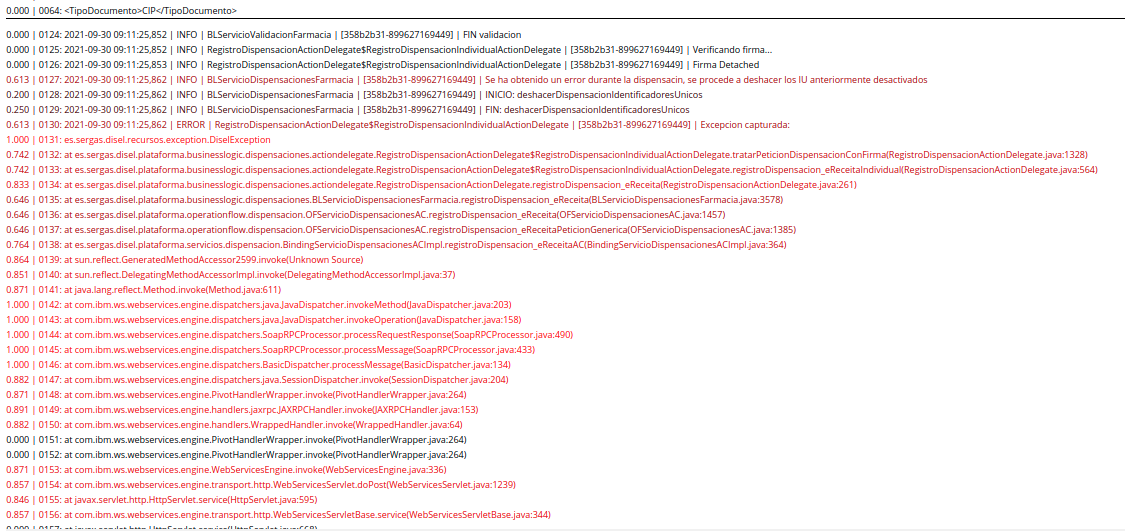
\includegraphics[width=15cm]{figuras/report.png}}
\caption{Ejemplo salida detección anomalías}
\label{enlace1}
\end{figure}


%
% Engadir os capitulos que fagan falta
%
\cleardoublepage
\chapter{Conclusiones y posibles ampliaciones}

\section{Conclusiones}

Se consideran las siguientes conclusiones acerca de los objetivos propuestos:

\begin{itemize}

\item \textbf{Manejo de los logs}: Se ha conseguido una forma correcta de manejar la cantidad de logs generada dotándola de sentido para el observador gracias la utilización del ELK Stack. Kivana proporciona posibilidades de generación de informes con el fin de ayudar a los responsables a obtener información relevante a partir de los registros de la aplicación.

\item \textbf{Generación de alertas}: teniendo en cuenta que el proceso de detección de alertas se está ejecutando sobre un entorno con una cantidad de datos inferior a la real es lo suficiente rápido como para que suponga una mejora en los servicios de operación de la aplicación. El uso de ElastAlert es lo suficientemente flexible como para generar las alertas necesarias y las operaciones asociadas.
Para asegurar este comportamiento se realizarían pruebas de rendimiento sobre entornos de preproducción con cantidades de datos semejantes a producción.

\item \textbf{Obtención de anomalías}: la aplicación de LogReduce sobre los registros de errores desconocidos genera informes en los que efectivamente se puede observar la causa raíz del error. En este punto se obtienen falsos positivos debido a la estructura compleja de los logs y a que existen un número muy grande de posibilidades, sin embargo, aún no siendo un resultado óptimo si que se considera una mejora en el proceso de revisión.

\end{itemize}


\section{Posibles ampliaciones}

\begin{enumerate}
\item \textbf{Servidor Cloud ejecutando ELK}: la arquitectura propuesta de ELK podría estar alojada en un entorno Cloud como podría ser Amazon Web Services (AWS) o Windows Azure o bien servidores propios interconectados entre si. Tendía sentido dividir los distintos elementos en diferentes máquinas, por ejemplo, añadir un elemento como FileBeat de forma local, que envíe la información de los logs a un LogStash remoto y este, a su vez, enviara los datos refinados a otra máquina que ejecutaría Elastic Search y Kibana. Se podría garantizar la visualización de los datos a través de Kibana en una url fija accesible desde equipos remotos.
\item \textbf{Alertas por picos de actividad o tiempos de respuesta altos}: a la hora de monitorizar la actividad aportaría valor el hecho del registro de eventos que suponen un peor rendimiento para la aplicación. Podrían ser tiempos de respuesta altos que no lleguen a ser TimeOuts o registrar picos de usuarios a ciertas horas que podrían para localizar momentos en los que se espera que podría producirse caídas.
\item \textbf{Detector de anomalías}: se podría plantear añadir un módulo que se encargue de validar los comportamientos normales de la aplicación, con el fin de localizar y minimizar el fraude de los responsables que utilizar la aplicación. 
\end{enumerate}


\cleardoublepage
\markboth{BIBLIOGRAFÍA}{BIBLIOGRAFÍA}
\addcontentsline{toc}{chapter}{Bibliografía}


\begin{thebibliography}{99}
% EXEMPLO DE DOCUMENTO DESCARGADO DA WEB
\bibitem{logstash} Logstash Reference ({\it https://www.elastic.co/guide/en/logstash/current/index.html}). Consultado el 1 de octubre de 2021.

\bibitem{elastic.co}
E. BV, elastic.co, Elasticsearch BV, 2021. [En línea]. Disponible:
https://www.elastic.co/guide/en/kibana/current/index.html. Consultado el 1 de octubre de 2021.

\bibitem{Libro 1}
Han, J. Kamber, M. Pei, J. Data Mining: Concepts and Techniques. Ed. 3,
Morgan Kaufmann Publishers Inc., 2003.

\bibitem{Libro 2}
Rich Collier, Bahaaldine Azarmi  Machine Learning with the Elastic Stack: Expert techniques to integrate machine learning with distributed search and analytics Ed. 1,
Packt Publishing, 2019.

\bibitem{logreduce}
Quiet log noise with Python and machine learning. [En línea]. Disponible:
https://opensource.com/article/18/9/quiet-log-noise-python-and-machine-learning
. Consultado el 1 de octubre de 2021.

\end{thebibliography}



\end{document}
